\section{Method/Implementation}

\subsection{Technical Setup}

The experimental environment was developed using React, a JavaScript library for building user interfaces, in combination with React Three Fiber (R3F), a React renderer for Three.js that enables declarative 3D scene construction in web browsers. This technology stack was chosen to create an accessible, browser-based reinforcement learning environment that requires no specialized software installation, making it suitable for educational purposes and broad accessibility.

The application architecture separates the game environment from the learning algorithm, allowing for both manual control through keyboard inputs and autonomous operation via the reinforcement learning agent. State management was implemented using Zustand, a lightweight state management solution, to handle real-time parameter adjustments and data collection throughout the training process.

\subsection{Environment Design}

\subsubsection{Game Environment}
The experimental environment implements a simplified Markov Decision Process where an agent, represented as a spherical object, must navigate along a straight path to reach a designated goal. The environment satisfies the Markov property as the agent's next state depends only on its current state and chosen action, not on the history of previous states. The level design features an open starting area behind the player's initial position and bounded sides along the forward path. This asymmetric boundary design was intentionally implemented to encourage forward movement while providing clear failure states that enable the agent to learn the consequences of suboptimal actions.

\subsubsection{Action Space}
The action space $A$ comprises four discrete actions available to the agent at each time step, forming the action component of the MDP framework: \textit{Forward, Backward, Jump, None}.

\subsubsection{State Representation}
The state space $S$ was discretized to enable tabular Q-learning implementation while maintaining the Markov property. The agent's state is characterized by:
\begin{itemize}
    \item Distance to goal (discretized into 20 bins)
    \item Vertical position (discretized into 3 bins to capture ground/air states)
\end{itemize}

This discretization ensures that each state contains sufficient information for optimal decision-making without requiring knowledge of previous states, thus preserving the fundamental assumption underlying the MDP formulation.

\subsubsection{Reward Structure}
The reward function $R(s,a,s')$ was designed to provide clear learning signals that guide the agent toward the optimal policy within the MDP framework:
\begin{itemize}
    \item \textbf{Goal Achievement}: +100 points for reaching the goal
    \item \textbf{Fall Penalty}: -10 points for falling off the level
    \item \textbf{Wall Collision}: -2 points for collision with boundaries
    \item \textbf{Time Penalty}: -0.1 points per time step to encourage efficient path completion
\end{itemize}

\subsubsection{Obstacle Configuration}
The environment initially included three obstacles positioned along the path, configurable as either fixed or randomly positioned elements. However, preliminary testing revealed that obstacle presence, particularly in random configurations, significantly impeded the learning process. Consequently, an obstacle toggle mechanism was implemented, with obstacles disabled by default to facilitate initial learning of the fundamental forward-movement behavior.

\subsection{Reinforcement Learning Algorithm}

\subsubsection{Exploration Strategy}
An $\varepsilon$-greedy exploration strategy was implemented to address the exploration-exploitation trade-off inherent in MDP solutions. This strategy ensures sufficient exploration of the state-action space to guarantee convergence to the optimal policy, as required by the theoretical foundations of Q-learning in finite MDPs. The exploration rate $\varepsilon$ begins at 1.0 (full exploration) and decays exponentially according to:

\begin{equation}
\varepsilon_{t+1} = \max(\varepsilon_{min}, \varepsilon_t \times 0.98)
\end{equation}
where $\varepsilon_{min} = 0.05$ represents the minimum exploration rate to maintain continued exploration throughout training.

This decay schedule ensures that early learning phases prioritize exploration of the MDP's state-action space, while later phases focus on exploitation of learned optimal actions, consistent with the convergence requirements for Q-learning in finite MDPs.

\subsubsection{Episode Structure}
Training proceeds through discrete episodes, where each episode begins with the agent at the starting position and terminates when one of the following conditions is met:
\begin{itemize}
    \item Goal achievement (successful episode)
    \item Agent falls off the level boundaries (failure episode)  
    \item Maximum step limit exceeded (timeout episode)
\end{itemize}

The Q-table is updated after each action-reward transition, and the exploration parameter is decremented after each completed episode.

\subsubsection{Parameter Configuration}
The learning algorithm utilizes the following hyperparameters, selected through empirical testing:
\begin{itemize}
    \item Learning rate ($\alpha$): 0.1
    \item Discount factor ($\gamma$): 0.95
    \item Initial exploration rate ($\varepsilon_0$): 1.0
    \item Minimum exploration rate ($\varepsilon_{min}$): 0.05
    \item Exploration decay rate: 0.98 per episode
\end{itemize}

\subsection{User Interface Design}

\begin{figure}[htbp]
    \centering
    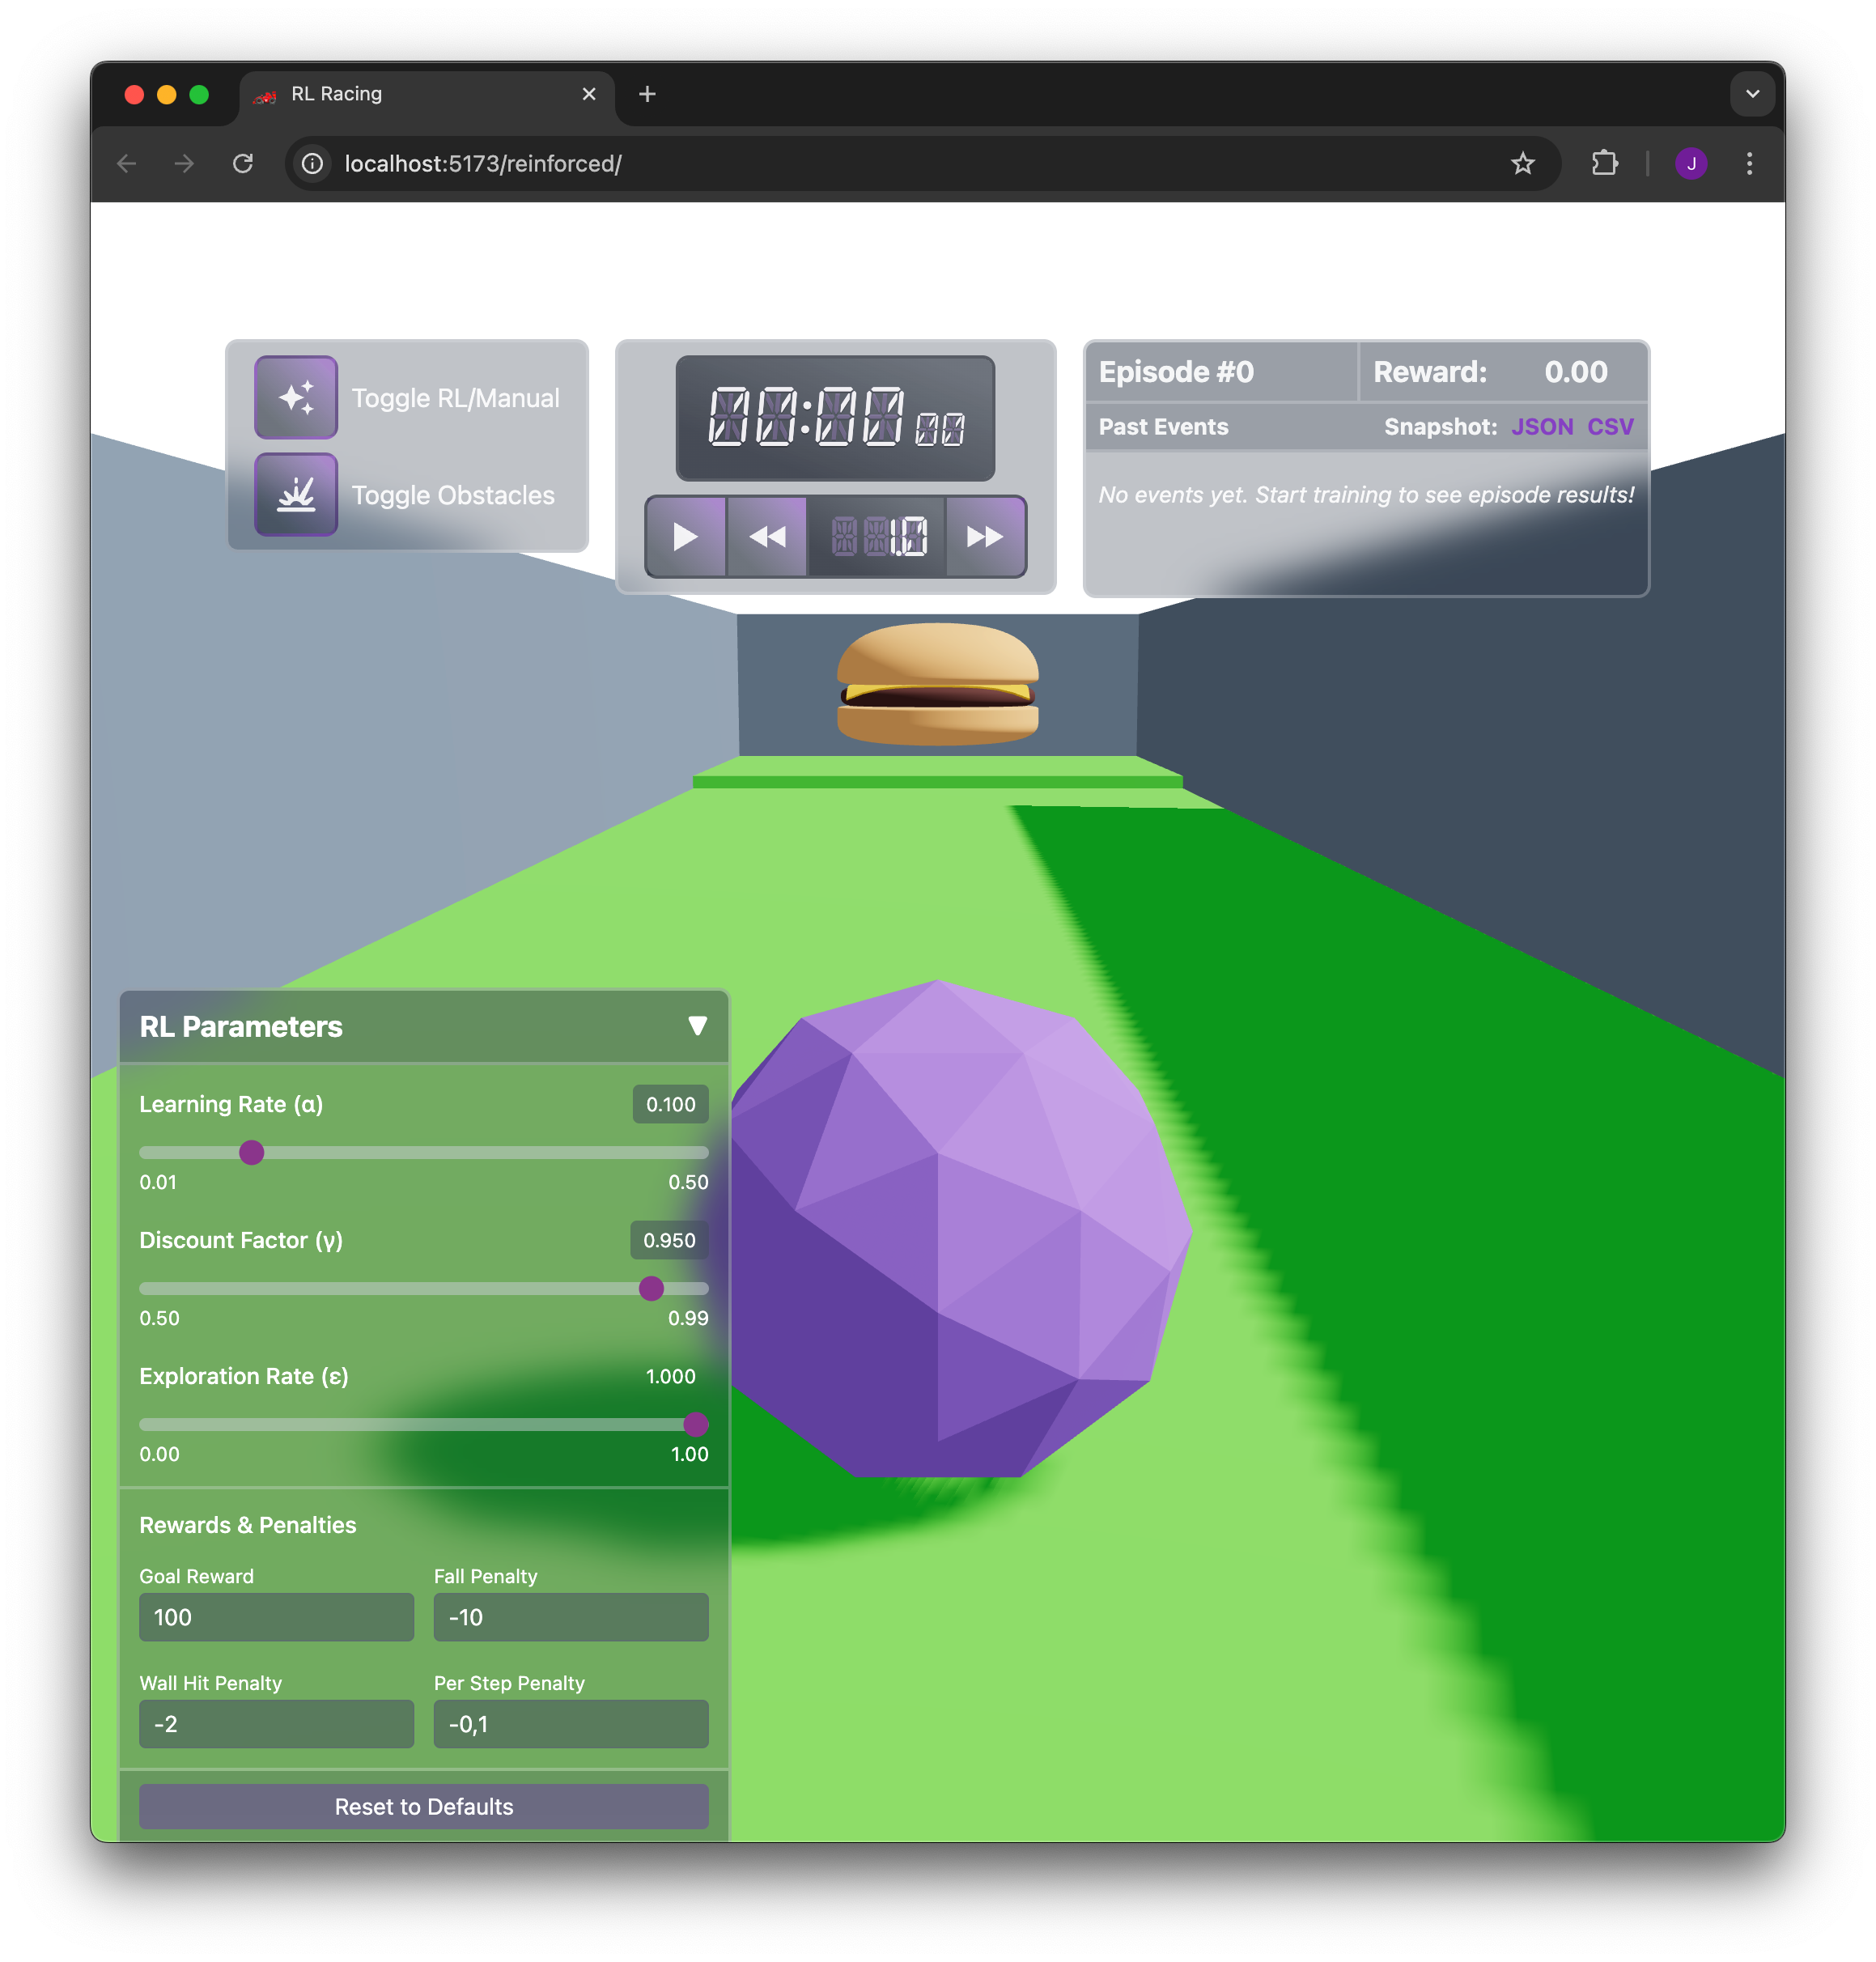
\includegraphics[width=0.45\textwidth]
    {figures/rl_racing_main.png}
    \caption{Final web application as seen on initial load.}
    \label{fig:rl_racing_main}
\end{figure}

The user interface was designed to provide intuitive control over fundamental reinforcement learning parameters and environmental conditions, enabling users to explore the impact of different configurations on agent behavior without requiring programming knowledge - Figure \ref{fig:rl_racing_main}.

\subsubsection{Real-time Monitoring Components}
A Timer component was implemented to display the duration of each episode in real-time. This component was initially designed as part of a broader simulation speed control system that would allow users to accelerate the learning process and observe long-term learning trends within compressed timeframes. However, due to technical complexity in synchronizing the physics simulation with variable time scales and project time constraints, the simulation speed control feature was not fully implemented in the final system.

The EventLogger component serves as a comprehensive monitoring system that displays real-time updates of total episode rewards alongside a chronological log of past episode outcomes. This component addresses the pedagogical need for immediate feedback by showing users the direct consequences of the agent's actions and parameter adjustments. The interface displays both the current episode's accumulated reward and a scrollable history of previous episodes, enabling users to identify learning trends and performance improvements over time.

\subsubsection{Dynamic Environment Control}
A critical educational feature of the interface is the obstacle toggle functionality, which allows users to enable or disable environmental obstacles at any point during the training process. This real-time environment modification capability demonstrates the impact of environmental complexity on learning performance, providing immediate visual evidence of how increased task difficulty affects agent behavior and learning progression.

\subsubsection{Data Export and Analysis Tools}
To facilitate deeper analysis of learning behavior, the system implements data export functionality that captures comprehensive training metrics in both JSON and CSV formats. The export system provides snapshot capabilities that allow users to download detailed learning data without interrupting the ongoing training process, preserving the real-time learning experience while enabling post-hoc analysis.